\documentclass[9pt]{beamer}
% \documentclass[notes, handout, 9pt]{beamer}
% \documentclass[handout, 9pt]{beamer}

\usepackage{import}
\subimport{../}{preamble.tex}
\subimport{../}{beamer-theme.tex}
\usepackage{svg}

% Location for all figures / pictures
\graphicspath{{pictures/}{figures/}}


% % Figures inline
\usepackage{tikz}
\usepackage{pgfplots}
\usetikzlibrary{calc}
\usetikzlibrary{shapes.multipart}
\usetikzlibrary{decorations.pathreplacing}
\usetikzlibrary{arrows.meta}
\usepgfplotslibrary{fillbetween}

%--------------------------------------------------
% Presentation Information
%--------------------------------------------------
\title[Continuous Optimization]{KKT Optimality Conditions}
\author[]{\textbf{Bart Van Parys}}
\date[]{Fall 2026}
%--------------------------------------------------

\begin{document}

\begin{frame}  

  \maketitle

  \vspace{-2em}
  
    \begin{center}
    \begin{tabular}{lll}
      Instructor : & \textbf{Bart Van Parys} & \textbf{(\href{mailto:mastermath@vanparys.xyz}{mastermath@vanparys.xyz})} \\
    \end{tabular}
  \end{center}
  
\end{frame}

\section{Unconstrained Optimality Conditions}

\begin{frame}{Unconstrained Optimality Conditions}

  \emph{Unconstrained optimization}: \quad
  \(
    \min_{x\in\Re^n} \,f(x)
  \)

  \vfill
  
  In earlier lectures we have proven the following:
  
  \vfill
  
  \textbf{(1) Theorem : } Let $f:\Re^n\to\Re$ be a continuously differentiable function. Then,
  \[
    x^\star \in \arg\min_{x\in \Re^n} f(x) \implies  f'(x^\star) =0.
  \]

  \vfill

  \textbf{(2) Theorem : } Let $f:\Re^n\to\Re$ be a continuously differentiable \emph{convex} function. Then,
  \[
    x^\star \in \arg\min_{x\in \Re^n} f(x) \iff  f'(x^\star) =0.
  \]

  \vfill

  \textbf{(3) Theorem : } Let $f:\Re^n\to\nRe$ be a \emph{convex} function. Then,
  \[
    x^\star \in \arg\min_{x\in \Re^n} f(x) \iff  \partial f(x^\star) \ni 0.
  \]

\end{frame}

\begin{frame}{Constrained Optimality Conditions}

  \emph{Constrained optimization}: \quad
  \[
    \begin{array}{rl}
      \min_{x\in\Re^n} & f(x) \\[0.5em]
      \st & g_i(x) \geq b_i \quad \forall i\in [1,\dots, m]
    \end{array}
  \]

  \vfill

  \uncover<2->{
  Vanishing gradient is clearly not relevant here!

  \vfill

  \textbf{Example:} Consider indeed
  \[
    \min \set{x}{x\geq 1}
  \]
  with $x^\star=1$ despite $f'(x^\star)=1$.
  }
\end{frame}

\section{Subdifferentials of Maxima and Aggregates}

\begin{frame}{Subdifferential of a sum}

  Let $f_1, f_2:\Re^n\to\nRe$ be lsc convex such that $D \defn \cap_{i} \relint(\dom(f_i))\neq \emptyset$ and $s\defn f_1+f_2$.

  \vfill
  \textbf{Theorem :}
  \[
    \partial s(x) = \partial f_1(x) + \partial f_2(x) \quad \forall x \in D
  \]

  The proof of the previous result is due to Rockafellar and is too complicated to discuss here. The direction $\supseteq$ is trivial. If $g_i\in \partial f_i(x)$, i.e.,
  \[
    f_i(y) \geq f_i(x) + \iprod{g_i}{y-x} ~~\forall x, ~\forall i,
  \]
  then evidently, $g_1+g_2\in\partial s(x)$.

  % \vfill
  % \textbf{Sketch $\subseteq$}: We use $g\in \partial s(x) \iff s(x) + s^\star(g)=\iprod{g}{x}$. It can be shown that $s^\star(g)=\inf\set{f_1^\star(u)+f_2^\star(v)}{u+v=g}$ when $D\neq \emptyset$. Now
  % \[
  %   g\in\partial s(x)\iff \iprod{g}{x}=f_1(x)+f_2(x) + f^\star_1(u^\star)+f_2^\star(v^\star), ~g=u^\star+v^\star
  % \]
  
\end{frame}


\begin{frame}{Subdifferential of a Maximum}

  Let $f_1, \dots, f_m : \Re^n\to\nRe$ be lsc convex such that $D \defn \cap_{i=1}^m \interior \dom(f_i) \neq \emptyset$. Let $f\defn \max_{i\in [1,\dots,m]} \, f_i$.

  \vfill

  \begin{minipage}{0.5\textwidth}
    \textbf{Danskin's Theorem : } Let $I(x) \defn \set{i}{f_i(x)=f(x)}$ for $x \in D$. Then,
    \[
      \partial f(x) = C \defn \conv \set{\partial f_i(x)}{ i \in I(x)}.
    \]
  \end{minipage}%
  \hfill
  \begin{minipage}{0.5\textwidth}
    \centering
    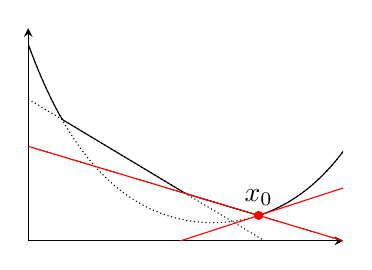
\begin{tikzpicture}
      \begin{axis}[
        ticks=none,
        axis lines=left,
        y=3cm,            % y unit vector
        x=1cm,            % x unit vector
        xmin=-2,
        xmax=2,
        ymin=0.1,
        ymax=1,
        clip=true
        ]
        
        \addplot[mark=none, black, samples=100, domain=-2:2] {max((exp(-x)+exp(x)/2)/8, 0.3 - 0.1*(x), 0.3 - 0.2*x)};
        \addplot[mark=none, densely dotted, black, samples=100, domain=-2:2] {0.3 - 0.2*x};
        \addplot[mark=none, densely dotted, black, samples=100, domain=-2:2] {0.3 - 0.1*x};
        \addplot[mark=none, densely dotted, black, samples=100, domain=-2:2] {(exp(-x)+exp(x)/2)/8};
        

        \node[circle, inner sep=1, draw=red, fill=red] (x0) at (axis cs:0.926522, 0.2073478) {};
        \node[above] at (x0) {\red{$x_0$}};

        \addplot[mark=none, red, samples=100, domain=-2:2] {0.2073478 - 0.1*(x-0.926522))};
        \addplot[mark=none, red, samples=100, domain=-2:2] {0.2073478 + 0.108366*(x-0.926522))};
        
        % \addplot+[thick, draw=blue, mark=none, fill=blue] coordinates {(-1,0.362777) (1.5, 0.307996) };
        
      \end{axis}
    \end{tikzpicture}
  \end{minipage}

\end{frame}

\begin{frame}{Proof}

  \textbf{Proof sketch [$\star$]:}
  \begin{itemize}
  \item As $\partial f(x)$ and $C$ are convex and closed we need that the support functions $\sigma_C = \sigma_{\partial f}$.
  \item Let $d \in \Re^n$. Then $\lim_{t\downarrow 0} I(x + td) \subseteq I(x)$.
  \item $\sigma_{\partial f(x)}(d) = \nabla f(x)[d] = \max_{i \in I(x)} \nabla f_i(x)[d]$.
  \item $\nabla f_i(x)[d] = \sigma_{\partial f_i(x)}(d) = \max \set{\iprod{g_i}{d}}{g_i \in \partial f_i(x)}$.
  \item $\sigma_C(d) = \sigma_{\partial f(x)}(d) = {\displaystyle\max_{i\in I(x)}} \set{\iprod{g_i}{d}\!\!}{\!\!g_i\in \partial f_i(x)} = {\displaystyle\max_{i\in I(x)}} \set{\iprod{g}{d}\!\!}{\!\!g\in \conv({\displaystyle \cup_{i\in I(x)}}\partial f_i(x))}$
  \end{itemize}

\end{frame}

% \begin{frame}{Subdifferential of a maximum} %

%   \textbf{Proof : }
%   \begin{itemize}
%   \item $\sigma_C = \sigma_{\partial f} \iff C = \partial f$ when $C$ and $\partial f$ are convex and closed. This result can be proven using separating hyperplanes as done in Homework 2. Consider indeed any sequence $\{g_i \in \partial f(x)\}_{i\geq 1}$ with limit $g$. Then, $\lim_{i\to \infty}\iprod{g_i}{y-x} + f(x) \leq f(y)$ for all $y$ implies by continuity of linear functions that $\iprod{g}{x-x_i} + f(x) \leq f(y)$ for all $y$ too. Hence, $g\in\partial f(x)$. As this holds for any converging sequence, $\partial f(x)$ is a closed set. The sets $\partial f_i(x) \subseteq B[0, L_i]$ are bounded as $f_i(x)$ is locally Lipschitz with constant $L_i$ (L3). The same argument as before shows that $\partial f_i(x)$ are closed too. The convex hull of compact sets is compact.
%   \end{itemize}
  
% \end{frame}


\section{Constrained Optimality Conditions}

\begin{frame}{The Karush-Kuhn-Tucker (KKT) Theorem}

  \begin{minipage}{0.33\textwidth}
    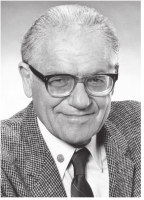
\includegraphics[height=3cm]{karush.png}\\
    Karush
  \end{minipage}%
  \hfill
  \begin{minipage}{0.33\textwidth}
    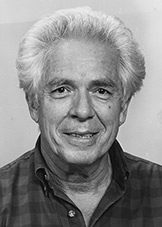
\includegraphics[height=3cm]{kuhn.jpg}\\
    Kuhn
  \end{minipage}%
  \hfill
  \begin{minipage}{0.33\textwidth}
    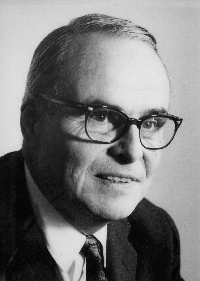
\includegraphics[height=3cm]{tucker.jpg}\\
    Tucker
  \end{minipage}%

  \vfill

  \begin{itemize}
    \setlength\itemsep{1em}
  \item Proven in 1939 in the master thesis of Karush. Rediscovered in 1951 by Kuhn and Tucker.
  \item Very important cornerstone in optimization
  \end{itemize}
  
\end{frame}


\begin{frame}{Karush-Kuhn-Tucker Theorem for Differentiable Functions}

  \uncover<2->{
  Let $f:\Re^n\to\Re$ and $g_1, \dots, g_m:\Re^n\to\Re$ be differentiable functions. A point $\bar x$ satisfies the linear independence constraint qualifications (LICQ) if 
  \[
    \set{g_i'(\bar x)}{i\in I(\bar x)}
  \]
  are linearly independent with $I(\bar x) \defn \set{i}{g_i(\bar x)=b_i}$.
}

  \vfill
  
  \textbf{Theorem :} Let $f:\Re^n\to\Re$ and $g_1, \dots, g_m:\Re^n\to\Re$ be continuously differentiable functions.
  Let $x^\star$ satisfy the LICQ condition and $x^\star\in \arg \min \{f(x)~ \st~ g(x)\succeq b\}$. Then,
  \[
  \begin{array}{rl}
    g(x^\star) \succeq b, & {\rm{Feasibility}}\\[0.5em]
    \lambda_i^\star\succeq 0 {\rm{~for~}} i \in [1, \dots, m]: &{\rm{Multipliers}} \\[1em]
    f'(x^\star) - \sum_{i \in I(x^\star)} \lambda_i^\star g'_i(x^\star) = 0 &
  \end{array}
  \]
  with $I( x^\star) \defn \set{i}{g_i(x^\star)=b_i}$.
\end{frame}

\begin{frame}{Mechanical Interpretation}

  Linear optimization
  \[
    \begin{array}{rl}
      \min & c\tpose x \\[0.5em]
      \st  & a_i\tpose x\geq b_i \quad \forall i \in [1,2,3]
    \end{array}
  \]

  Take
  \begin{itemize}
  \item $c$: anti-gravity.
  \item $x$: the position of a small ball.
  \item $a_i\tpose x\geq b_i$: immovable walls.
  \item $p_i a_i$: force exerted from wall on ball.
  \end{itemize}
  
  \vfill

  \begin{center}
    \includesvg[height=4cm]{kkt.svg}
  \end{center}
  
\end{frame}

\begin{frame}{Example (LICQ)}

  \begin{center}
    \includegraphics[height=5cm]{licq/licq.pdf}
  \end{center}

  \vfill
  
  \textbf{Example:}
  \[
    \begin{array}{rl}
     (-\sqrt{2}, 0) = \arg \min & x_1+x_2 \\[0.5em]
      \st  & 2- x_1^2-x_2^2\geq 0,\\[0.5em]
           & x_2\geq 0
    \end{array}
  \]
  
\end{frame}

\begin{frame}{Example (no LICQ)}

  \begin{center}
    \includegraphics[height=5cm]{no-licq/no-licq.pdf}
  \end{center}

  \vfill
  
  \textbf{Example:}
  \[
    \begin{array}{rl}
     (0, \sqrt{2}) = \arg \min & x_1+x_2 \\[0.5em]
      \st  & 2- x_1^2-x_2^2\geq 0,\\[0.5em]
           & x_2\geq \sqrt{2}
    \end{array}
  \]
  
\end{frame}

\begin{frame}{The Karush-Kuhn-Tucker Theorem for Convex Functions}

  \uncover<2->{
    Let $f:\Re^n\to\Re$ be a convex function, $g_1, \dots, g_m$ be concave functions, $b\in \Re^m$ such that \emph{Slater's condition} holds:
    \[
      \exists \bar x : g_i(\bar x) > b_i
    \]
    for $i$ in $[1, \dots, m]$.
  }
  \vfill
  
  \textbf{Theorem :} Let the feasible set $\set{x}{g(x)\succeq b}$ satisfy Slater's constraint qualification.
  A point $x^\star$ is an optimal point of $\min \{f(x)~ \st~ g(x)\succeq b\}$ \emph{if and only if}
  \[
  \begin{array}{rl}
    g(x^\star) \geq b, & {\rm{Feasibility}}\\[0.5em]
    \lambda_i^\star\succeq 0 {\rm{~for~}} i \in [1, \dots, m]:  & {\rm{Multipliers}} \\[1em]
    \exists h_0 \in \partial f(x^\star), ~h_i\in\partial(- g_i(x^\star)) : h_0 + \sum_{i \in I(x^\star)} \lambda_i^\star h_i = 0 &
  \end{array}
  \]
  where $I(x^\star) \defn \set{i}{g_i(x^\star)=b_i}$.
  
\end{frame}

\begin{frame}{Proof using Subdifferentials}

  \[
    f^\star  = \min\set{f(x)}{x\in \Re^n, ~g(x)\succeq b}
  \]

  \vfill

  \textbf{Proof : }
  \begin{itemize}
    \setlength\itemsep{1em}
  \item Let $\phi(x)\defn \max \{f(x) - f^\star, b_1 - g_1(x), \dots, b_m-g_m(x)\}$ a convex function.
  \item<2-> $x^\star$ is a minimizer $\iff$ $x^\star \in \arg \min_x \phi(x)$ $\iff$ $0\in \partial \phi(x^\star)$ $\iff$ $0 \in \conv(\set{\partial f(x^\star), \partial (- g_i(x^\star)) }{i \in I(x^\star)})$ (indeed $f(x^\star)=f^\star$) $\iff$ $\exists h_0 \in \partial f(x^\star)$ and $h_i \in \partial (-g_i(x^\star))$, $\alpha_i\geq 0$ such that $\alpha_0+\sum_{i=1}^m \alpha_i=1$ and $0 = \alpha_0 h_0 + \sum_{i\in I(x^\star)} \alpha_i h_i$.
  \item<3-> $\alpha_0\neq 0$. First $\iprod{h_i}{y-x^\star} \leq g_i(x^\star) -g_i(y) = b_i - g_i(y)$ for all $y$ and $i \in I(x^\star)$. If $\alpha_0=0$ then contradiction $0 = \sum_{i\in I(x^\star)} \alpha_i \iprod{h_i}{\bar x - x^\star} \leq \sum_{i\in I(x^\star)} \alpha_i (b_i - g_i(\bar x))<0$ as $\sum_{i\in I(x^\star)} \alpha_i=1$ and $g_i(\bar x)>b_i$ satisfied by the Slater point $\bar x$.
  \item<4-> Simply take $\lambda_i^\star \defn \frac{\alpha_i}{\alpha_0}$.
  \end{itemize}
  
\end{frame}

\begin{frame}{Example (no Slater as well)}

  \begin{center}
    \includegraphics[height=5cm]{no-licq/no-licq.pdf}
  \end{center}

  \vfill
  
  \textbf{Example:}
  \[
    \begin{array}{rl}
     (0, \sqrt{2}) = \arg \min & x_1+x_2 \\[0.5em]
      \st  & 2- x_1^2-x_2^2\geq 0,\\[0.5em]
           & x_2\geq \sqrt{2}
    \end{array}
  \]
  
\end{frame}


\begin{frame}{The Karush-Kuhn-Tucker Theorem}

  Let $f:\Re^n\to\nRe$ be a convex function, $g_1, \dots, g_m$ be concave functions, $b\in \Re^m$ such that \emph{Slater's condition} holds:
  \[
    \exists \bar x : g_i(\bar x) > b_i
  \]
  for $i$ in $[1, \dots, m]$.

  \vfill

  \textbf{Theorem :} A point $x^\star$ is an optimal point of $\min \{f(x)~ \st~ g(x)\succeq b\}$ \emph{if and only if}
  \[
  \begin{array}{rl}
    g(x^\star) \geq b, & {\rm{Feasibility}}\\[0.5em]
    \lambda_i^\star\geq 0 {\rm{~for~}} i \in [1, \dots, m]:  & {\rm{Multipliers}} \\[1em]
    \exists h_0 \in \partial f(x^\star), ~h_i\in\partial(- g_i(x^\star)) : h_0 + \sum_{i\in[1,\dots,m]} \lambda_i^\star h_i = 0 &
  \end{array}
  \]
  where $\lambda_i^\star (b_i-g_i(x^\star)) =0$ for all $i$ (\emph{Complementarity}).
  
\end{frame}

\begin{frame}{KKT and Duality}

  What is the connection between KKT and duality?

  \vfill
  
  \begin{tcolorbox}
    Slater's condition $\implies$ strong duality
  \end{tcolorbox}

  \vfill

  \uncover<2->{
    \begin{tcolorbox}
      A KKT point $\implies$ strong duality
    \end{tcolorbox}
  }

\end{frame}

\begin{frame}{KKT and Duality}


  \[
    \begin{array}{rlcrl}
      \inf_x & f(x)  & \geq & \sup_F & F(b) \\[0.5em]
      \st & x\in X   & &                       \st & F \in \mc F(\Re^m_+) \\[0.5em]
             & g(x) \succeq b &&    & F(g(x)) \leq f(x), ~~\forall x \in X.
    \end{array}
  \]

  \vfill

  
  Suppose that $(x^\star, \lambda^\star)$ satisfy KKT system.
  We take as primal candidate $x^\star$ and as dual candidate $F^\star: c \mapsto \iprod{\lambda^\star}{c} + u_0$ with $u_0 = f(x^\star) - \iprod{\lambda^\star}{b}$.

  \vfill

  \begin{itemize}
  \item<2-> By direct substitution, we have $F^\star(b) = f(x^\star)$.
  \item<3-> $F^\star$ is feasible, i.e., $F^\star(g(x)) \leq f(x)$ for all $x$. Fix $x\in \Re^n$. First, $f(x^\star) \leq f(x) - \iprod{h_0}{x-x^\star} = f(x) + \sum_{i\in I(x^\star)} \lambda_i^\star \iprod{h_i^\star}{x-x^\star} \leq f(x) + \sum_{i\in I(x^\star)} \lambda_i^\star (g_i(x^\star)-g_i(x)) = f(x) + \sum_{i\in I(x^\star)} \lambda_i^\star (b_i - g_i(x))$, which is equivalent to $F^\star(g(x))\leq f(x)$ for all $x$.
  \end{itemize}

  \vfill

  \uncover<3->{
  Hence, \emph{strong duality} holds with $f(x^\star)=F^\star(b)$.
  }
\end{frame}

% \begin{frame}{A geometric view of KKT}

%   \begin{itemize}
%   \item For unconstrained convex optimization problems, we recover optimality condition
%     \begin{align*}
%       x^\star\in\arg\min_{x\in \Re^n} f(x) \iff &  0 \in \partial f(x^\star)\\
%       (\rm{differentiable~} f)\iff & \iprod{f'(x^\star)}{y-x^\star} \geq 0 \quad \forall y.
%     \end{align*}
%   \item<2-> When $f$ is differentiable and $X = \set{x}{g(x)\geq b}$ satisfies Slater's condition,
%     \[
%       \hspace{1.5em}x^\star\in\arg\min_{~x\in X~} f(x)\, \iff \iprod{f'(x^\star)}{y-x^\star} \geq 0 \quad \forall y \in X
%     \]
%   \end{itemize}

%   \vfill

%   \uncover<3->{
%     \textbf{Proof :}

%     KKT says that $f'(x^\star) = -\sum_{i \in I(x^\star)} \lambda_i^\star h_i$ with $\iprod{h_i}{y-x^\star} \leq g_i(x^\star)-g_i(y) = b_i - g_i(y)$ and $\lambda^\star_i\geq 0$ for any $i$ in $I(x^\star)$. Thus, $$\iprod{f'(x^\star)}{y-x^\star} = - \sum_{i\in I(x^\star)} \lambda_i^\star \iprod{h_i}{y-x} \geq \sum_{i\in I(x^\star)} \lambda_i^\star (g_i(y)-b_i) \geq 0$$ for all feasible $y$. The other direction follows from gradient inequality.
%   }
% \end{frame}

\section{Mechanics Interpretation [$\star$]}

\begin{frame}{M\'ecanique analytique}

  \begin{center}
    \includesvg[width=0.5\textwidth]{mass-spring.svg}
  \end{center}
  
  \vfill

  Lagrangian mechanics (``M\'ecanique analytique, 1788''), i.e.,
  \[
    \begin{array}{rl}
      \min & E(x_1, x_2) = \frac{k_1 x_1^2}{2} + \frac{k_2 (x_2-x_1)^2}{2} + \frac{k_3 (l-x_2)^2}{2}\\[0.5em]
      \st & x_1 - \frac{w}{2}\geq 0, \\[0.5em]
           & x_2-x_1 \geq w, \\[0.5em]
           & -x_2 - \frac{w}{2} \geq -l.
    \end{array}
  \]
  Nature optimizes for energy.
  
\end{frame}

\begin{frame}{KKT: Mechanics Interpretation}

  \begin{center}
    \includesvg[width=0.9\textwidth]{force-analysis.svg}
  \end{center}
  
  \vfill

  KKT system: 
  \[
    \begin{array}{lr}
      \lambda^\star_1, \lambda^\star_2, \lambda^\star_3 \geq 0, & \rm{Dual~variables}\\[1em]
      x^\star_1 - \frac{w}{2}\geq 0, ~x^\star_2-x^\star_1 - w \geq 0 ,~ -x^\star_2 - \frac{w}{2} + l\geq 0, & \rm{Feasibility}\\[1em]
      k_1 x_1^\star - k_2(x_2^\star-x_1^\star) - \lambda^\star_1 + \lambda^\star_2 = 0 & \rm{Mass~1} \\[1em]
      k_2 (x_2^\star-x_1^\star) - k_3 (l-x_2^\star) -\lambda^\star_2 + \lambda_3^\star = 0 & \rm{Mass~2} \\[1em]
      \lambda_1^\star(x^\star_1 - \frac{w}{2})=0, ~\lambda_2^\star(x^\star_2-x^\star_1 - w)=0, ~\lambda_3^\star(-x^\star_2 - \frac{w}{2} + l) = 0 & \rm{Complementarity}
    \end{array}
  \]

\end{frame}

\end{document}
%%% Local Variables:
%%% mode: latex
%%% TeX-master: t
%%% End:
